\section{GrainLearning evaluation}\label{section:GLPerformance} 

\begin{table}[H]
    \centering
    \begin{tabular}{l|lll|lll}
    Material                & \multicolumn{3}{l|}{Quartz Sand}       & \multicolumn{3}{l}{Limestone}          \\ \hline
    Attempt                 & 1          & 2           & 3           & 1          & 2           & 3           \\ \hline
    Restitution Coefficient & {[}0  1{]} & {[}0  1{]}  & {[}0 1{]}   & {[}0  1{]} & {[}0  1{]}  & {[}0 1{]}   \\
    Rolling Friction        & {[}0 1{]}  & {[}0 0.5{]} & {[}0.5 1{]} & {[}0 1{]}  & {[}0 0.5{]} & {[}0.5 1{]} \\
    Sliding Friction        & {[}0 1{]}  & {[}0 0.5{]} & {[}0.5 1{]} & {[}0 1{]}  & {[}0 0.5{]} & {[}0.5 1{]} \\
    Bond number             & {[}0 1{]}  & {[}0 0.5{]} & {[}0.5 1{]} & {[}0 1{]}  & {[}0 0.5{]} & {[}0.5 1{]} \\
    \end{tabular}
    \caption{Calibration attempts using GL}\label{table:GLCalibration}
\end{table}
                                        
\subsection{Limestone}
In the first and second calibration set of limestone, the clustering ability of GrainLearning is demonstrated~-~especially on the second one, as shown on Fig.~\ref{fig:Eskal}. 
\begin{figure}[H]
    \centering
    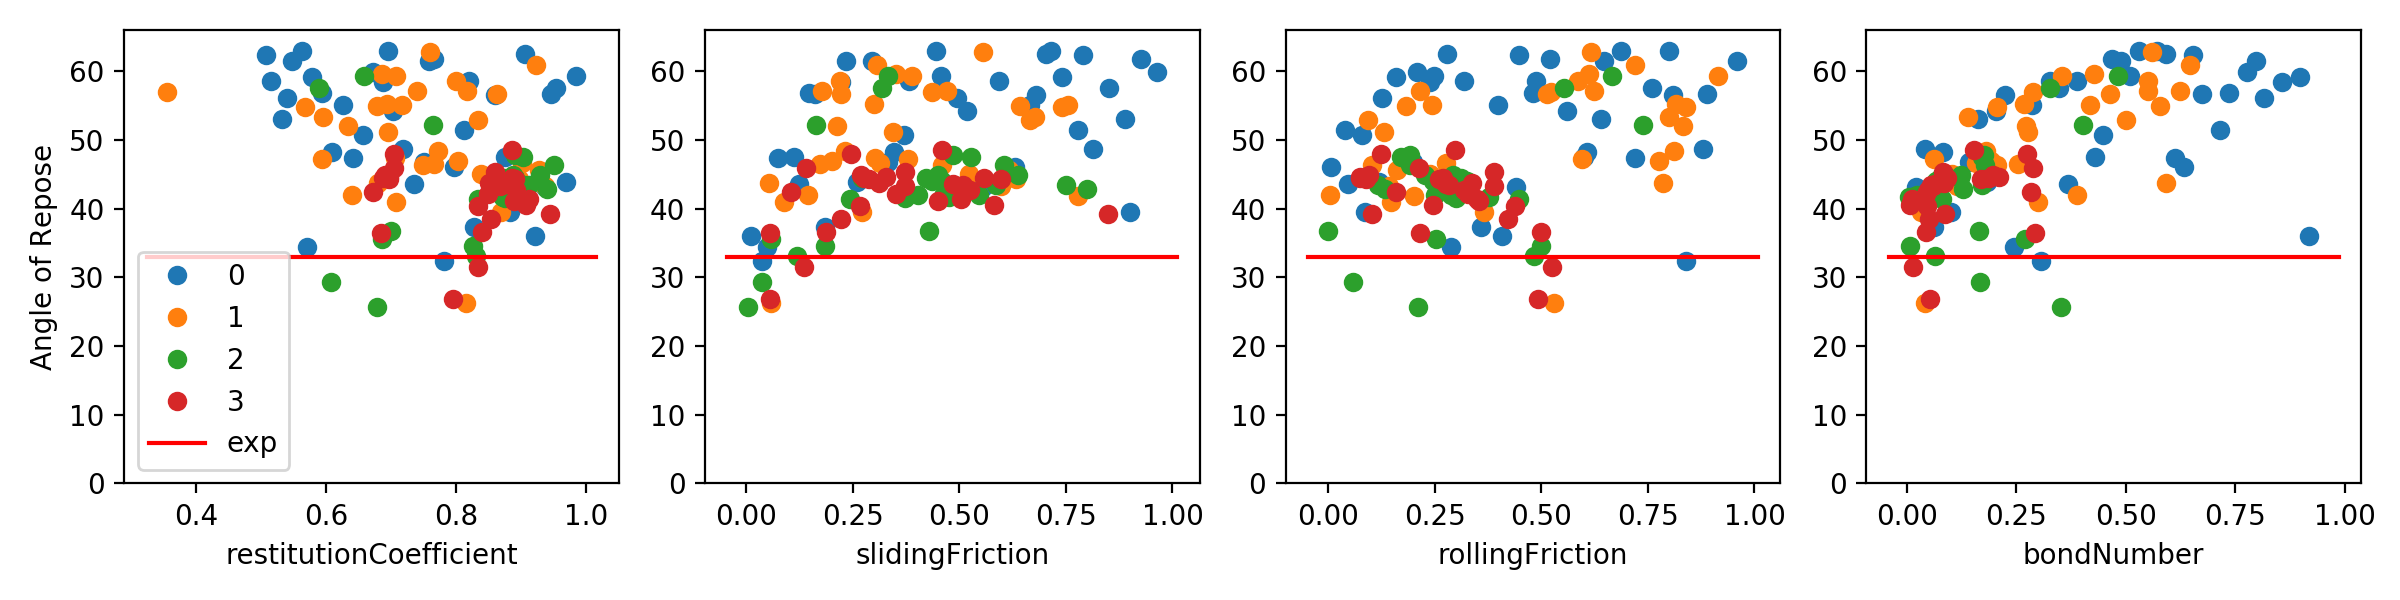
\includegraphics[scale=0.51]{ParametersObserver_Eskal150.png}
    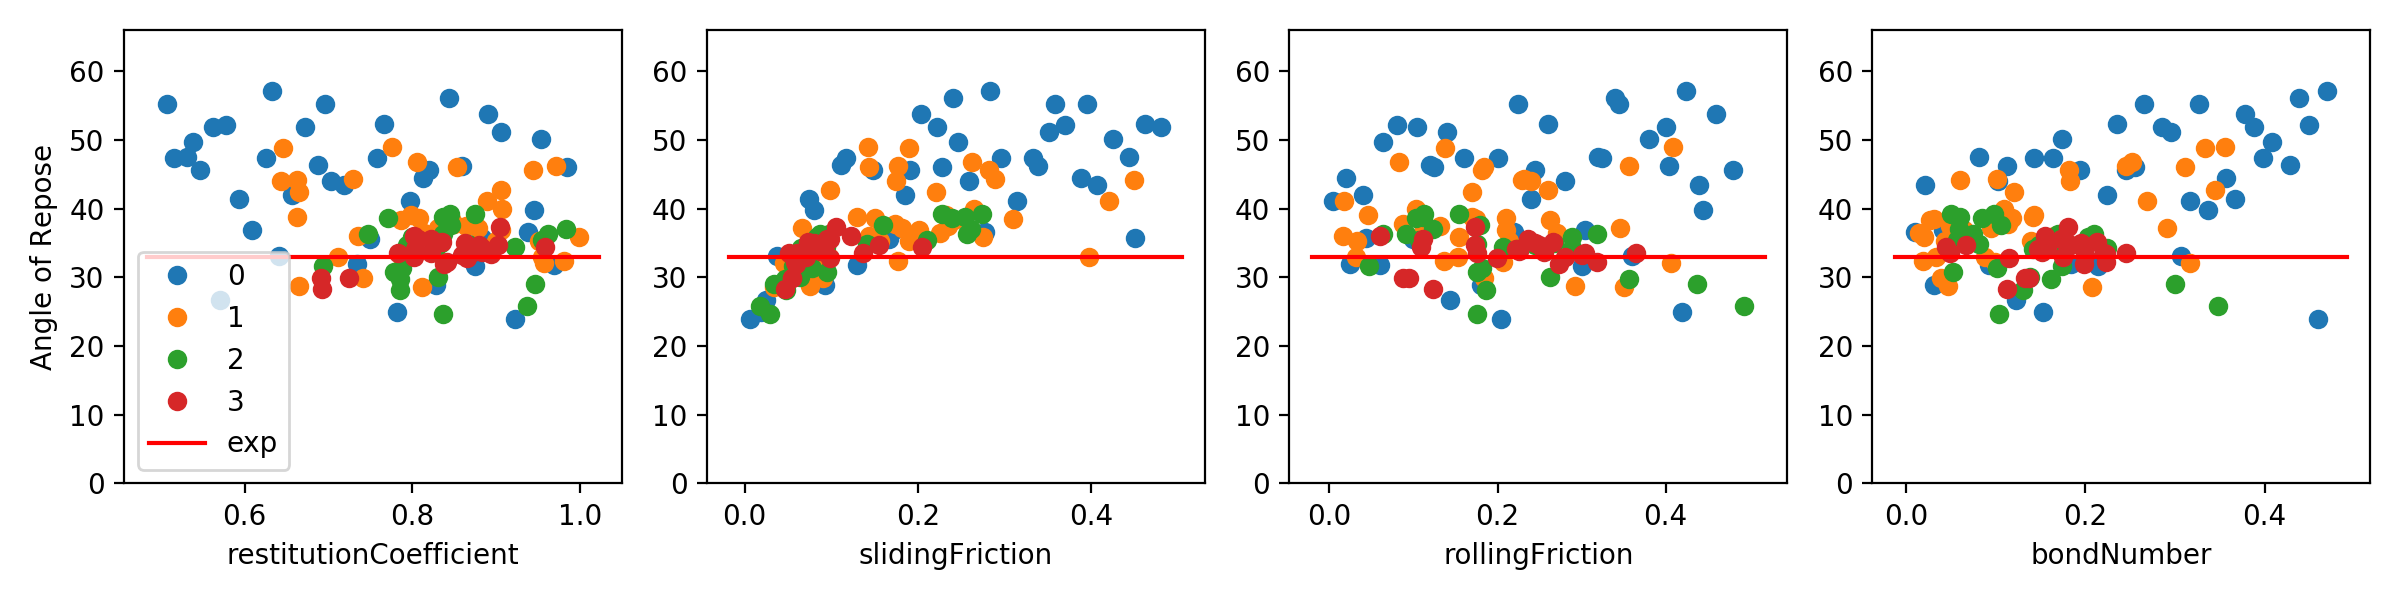
\includegraphics[scale=0.51]{ParametersObserver_Eskal150_1.png}
    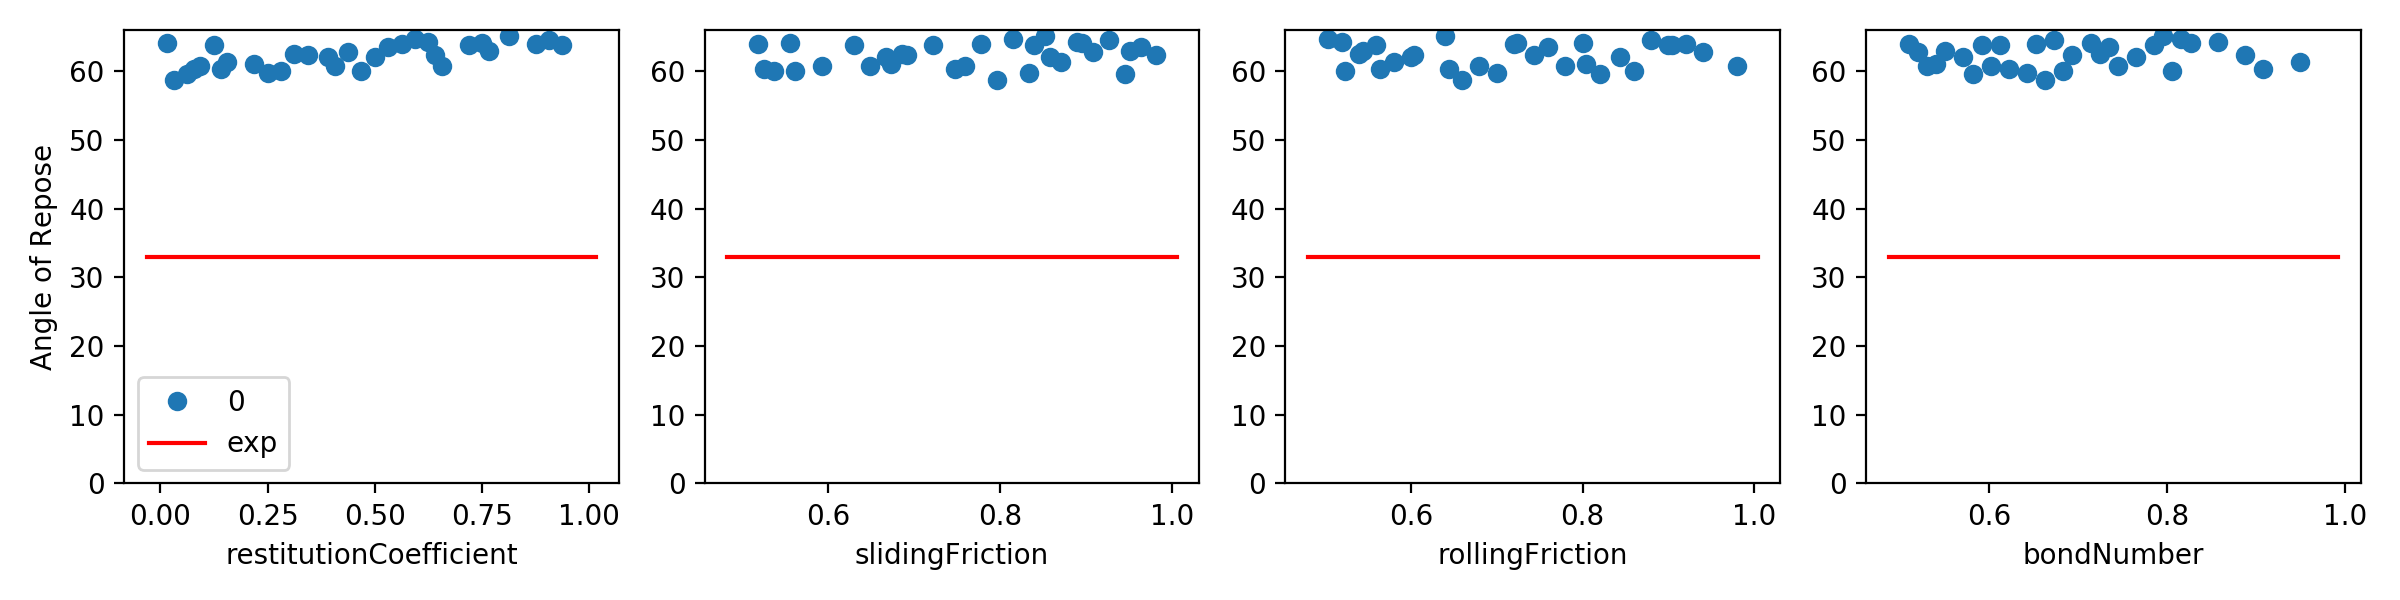
\includegraphics[scale=0.51]{ParametersObserver_Eskal150_2.png}
    \caption{\textit{From top to bottom,} attempt 1, 2, and 3 at calibrating Eskal with GL.\@ Scatter dots with different colors denote each iteration, and red line denotes experimental value.}\label{fig:Eskal}
\end{figure}


\subsection{Quartz sand}

\begin{figure}[H]
    \centering
    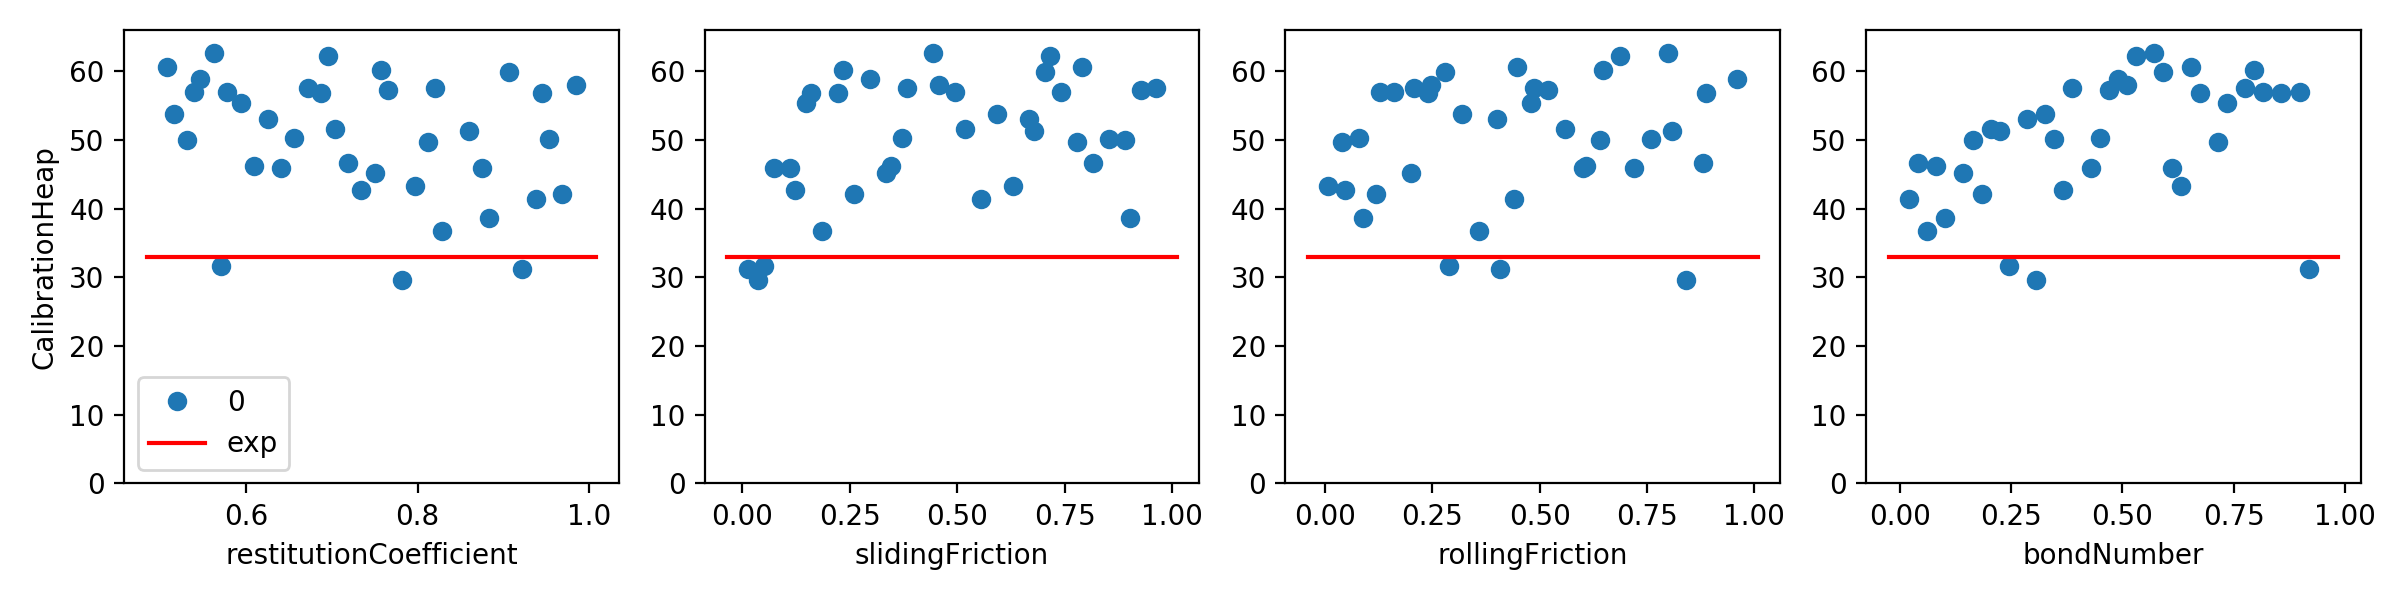
\includegraphics[scale=0.51]{ParametersObserver_SandHeap_copy.png}
    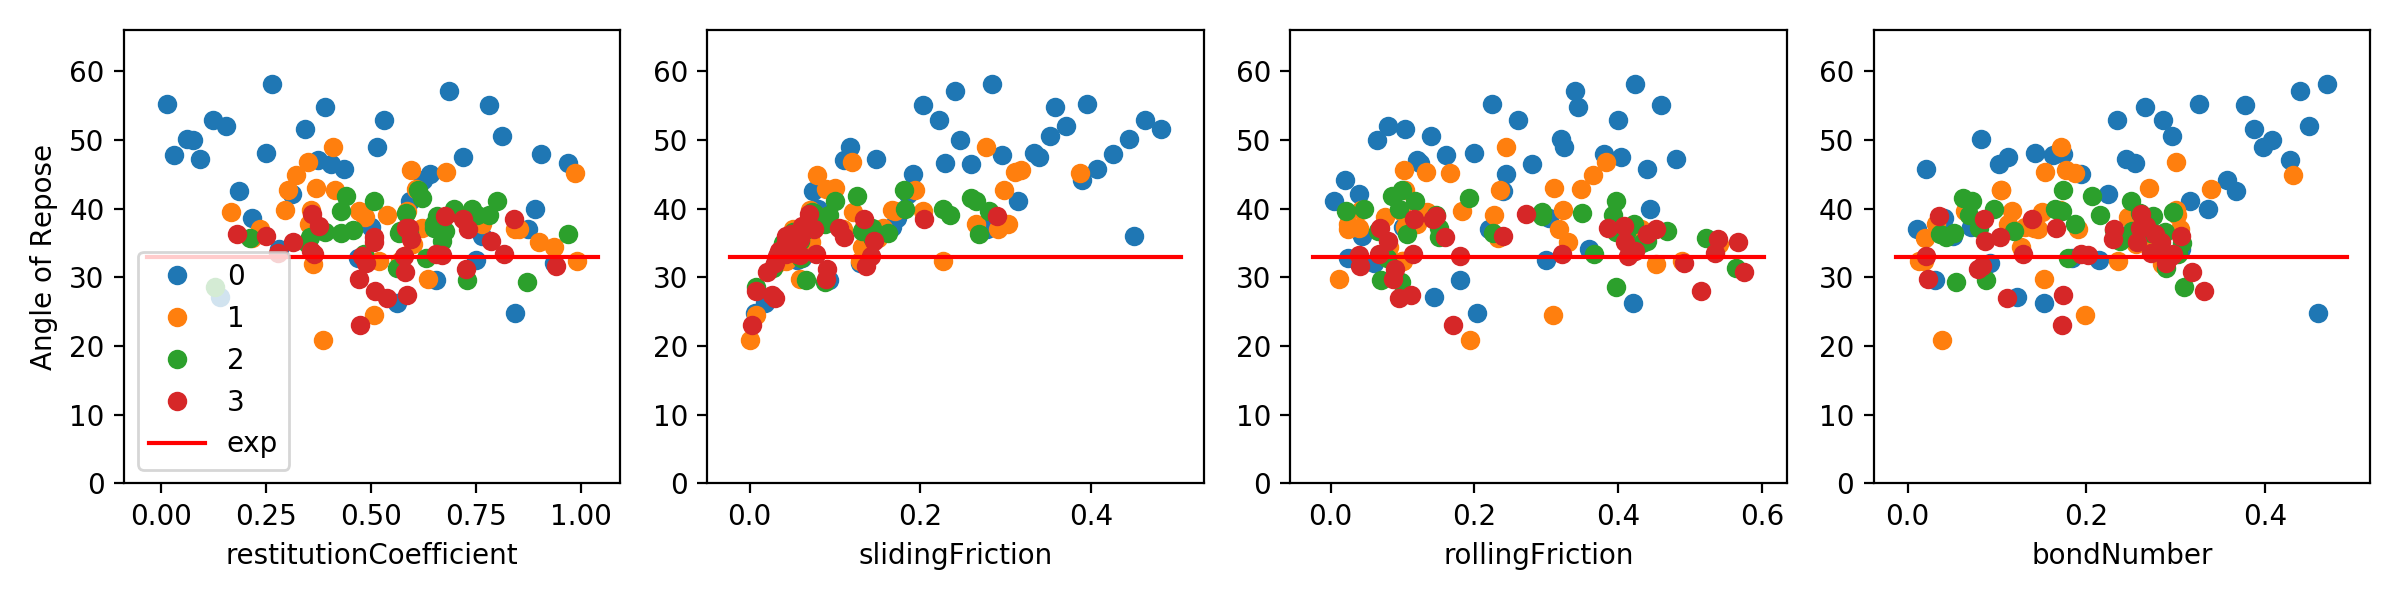
\includegraphics[scale=0.51]{ParametersObserver_Sand2.png}
    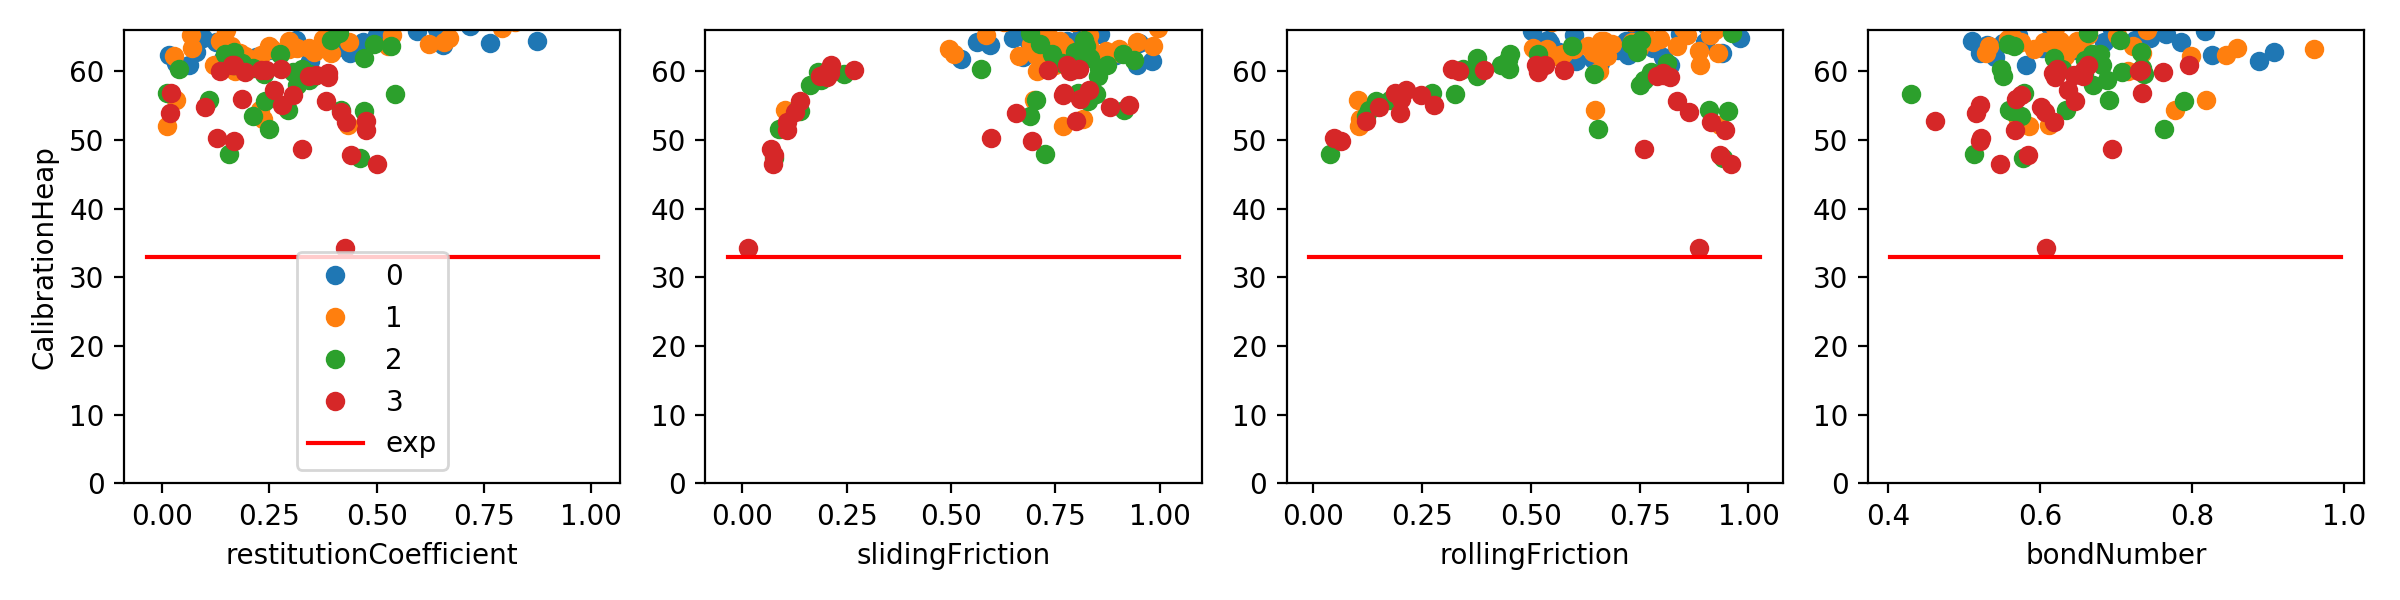
\includegraphics[scale=0.51]{ParametersObserver_Sand2_2.png}
    \caption{\textit{From top to bottom,} attempt 1, 2, and 3 at calibrating quartz sand with GL.\@ Scatter dots with different colors denote each iteration, and red line denotes experimental value.}\label{fig:Quartz}
\end{figure}



Throughout multiple calibration routines with GrainLearning, it is identified that the initial guessing range played a key role in the ability of GL to idenfity the correct set of micro-parameters. 


